\section{Serre equation}
\label{sec:Serre}

\subsection{The model}

\indent The Serre equations are a model to describe highly nonlinear waves propagating in shallow waters. Considering a horizontal bottom, these equations are written as

\begin{equation}
\label{eq:SerreFull}
h_t + (hu)_x = 0 \\
u_t + uu_x + gh_x - \frac{1}{3h}\left(h^3 \left( u_{xt} + uu_{xx} - (u_x)^2  \right) \right)_x = 0
\end{equation}

\noindent where $u = u(x,t)$, $h = h(x,t)$ and $g$ are, respectively, the depth-averaged horizontal velocity of the fluid, the water depth and the gravity acceleration. This formulation is based on \cite{CarterCienfuegos2011}.

\subsection{Discretization}

\indent As done previously for the numerical resolution of the KdV and the BBM equations, the Serre equations will be numerically solved using a splitting method, in which the system of equations will be decomposed in two : the first one will contain the advection terms, and the second one, all the high-order derivative terms.

\indent Therefore, the numerical resolution will consist in solve, in each time step $[t_n, t_{n+1}]$, the following problem :

\begin{equation}
\label{eq:SerreSplit1}
\begin{cases}
\th_t + \left(\th\tu\right)_x = 0 \\
\tu_t + \tu\tu_x + g\th_x = 0, \ \, t \in [t_n, t_{n+1}], \ \  (\th,\tu)(x,t_n) = (h,u)(x,t_n)
\end{cases}
\end{equation}

\begin{equation}
\label{eq:SerreSplit2}
\begin{cases}
\lh_t   = 0 \\
\lu_t - \frac{1}{3\lh}\left(\lh^3 \left( \lu_{xt} + \lu\lu_{xx} - (\lu_x)^2  \right) \right)_x = 0, \ \, t \in [t_n, t_{n+1}], \ \  (\lh,\lu)(x,t_n) = (\th,\tu)(x,t_{n+1})
\end{cases}
\end{equation}

\begin{equation}
\begin{cases}
(h,u)(x,t_{n+1}) = (\lh,\lu)(x,t_{n+1})
\end{cases}
\end{equation}

\indent If we denote the two systems by the operators $T_a^{\Delta t}$ and $T_d^{\Delta t}$, respectively, where the superscript indicates that the operator is performed over a time step $\Delta t$, the problem can be written as

\begin{equation}
(h,u)(x,t_{n+1}) = T_d^{\Delta t} \left( T_a^{\Delta t} \left((h,u)(x,t_n) \right) \right)
\end{equation}

\indent Some variations of the splitting scheme were also implemented. For example, inverting the order of the operators; or the method known as "strang splitting", in which three problems are solved in each time-step :

\begin{equation}
(h,u)(x,t_{n+1}) = T_a^{\frac{\Delta t}{2}} \left( T_d^{\Delta t} \left( T_a^{\frac{\Delta t}{2}} (h,u)(x,t_n) \right) \right)
\end{equation}

\noindent In the following descriptions of the resolution of the two schemes, the tilde and the overbar will be omitted for the sake of clarity.

\subsubsection{First system of equations (advection step)}

\noindent In order to solve the advection system (\ref{eq:SerreSplit1}) with the Roe solver (an approximation of the Riemman solver), one must write it in the classical form $U_t +  F(U)_x = 0$, where $U$ is the vector of unknowns and $F$ is a flux function.

\noindent We have that

\begin{equation}
\begin{split}
(hu)_t = uh_t + hu_t = -u(hu)_x - h\left(uu_x + gh_x\right) = -u\left (h_xu + 2hu_x \right) - ghh_x = \\ 
-\left(hu^2\right)_x - \frac{1}{2}g\left(h^2\right)_x = - \left(hu^2 +  \frac{1}{2}gh^2 \right)_x
\end{split}
\end{equation}

\noindent Therefore, the system can be rewritten as

\begin{equation}
\begin{cases}
h_t + \left(hu \right)_x = 0 \\
\left(hu \right)_t + \left(hu^2 +  \frac{1}{2}gh^2 \right)_x = 0
\end{cases}
\end{equation}

\noindent and we will solve it for the unknowns $U = \Atwo{h}{hu}$, with the flux function $F \Atwo{h}{hu} = \Atwo{hu}{hu^2 +  \frac{1}{2}gh^2} $. The time step is discretized using a 4th order Runge-Kutta scheme. The Riemman problem in each cell interface will be solved with the Roe solver (an approximated Riemman solver) associated with the MUSCL scheme for the reconstruction of the solution in the interfaces, giving a second order in space. 

\subsubsection{Second system of equations (dispersive step)}

\indent In the second system (\ref{eq:SerreSplit2}) of the splitted Serre equations , the water depth $h$ is constant in time, and therefore only the velocity $u$ must be updated. Separating the terms containing time derivatives, the second equation of thi suystem can be rewritten as 

\begin{equation}
\label{eq:dispersive}
\left( u - hh_xu_x - \frac{1}{3}h^2u_{xx} \right)_t  - \frac{1}{3h}\left(h^3 \left( uu_{xx} - (u_x)^2  \right) \right)_x = 0
\end{equation}

\indent This equation will be solved using an explicit Finite Difference scheme. Defining

$$g_1 = h^3 \left( uu_{xx} - (u_x)^2 \right)$$

$$g_2 = u - h h_x u_x - \frac{1}{3}h^2 u_{xx}$$

\noindent where the derivatives are evalueated using appropriate finite difference approximations.

\indent With this notation, using an one-step forward time discretization, one gets

$$(g_2)_i^{n+1} = (g_2)_i^n + \frac{\Delta t}{3h_i^n} \left(\left( g_1 \right)_x\right)_i^n = G_i^n$$

\noindent where the superscript and the subscript denotes respectively the time step and the spatial position.

\indent Using 2nd order centered approximation for the spatial derivatives in $(g_2)_i^{n+1}$, one gets the following tridiagonal linear system :

$$\left( \frac{h_i^n(h_x)_i^n}{2\Delta x} - \frac{(h_i^n)^2}{3\Delta x^2} \right)u_{i-1}^{n+1} + 
 \left( 1 + \frac{2(h_i^n)^2}{3\Delta x^2} \right)u_{i}^{n+1} + 
 \left( -\frac{h_i^n(h_x)_i^n}{2\Delta x} - \frac{(h_i^n)^2}{3\Delta x^2} \right)u_{i+1}^{n+1} = G_i^n $$
 
\noindent with the appropriate modifications to take in account the boundary conditions.
 
 
\paragraph{Alternative resolution of the second system (for the variables $(h,hu)$)}
 
\indent Inspired by the discretization described in \cite{Bonneton2011}, we will rewrite the second system of equations obtained in the splitting of the Serre equations, in order to solve it in the variables $(h,hu)$ and thus keep the formulation of the first system.
 
\indent For this purpose, we will multiply the equation (\ref{eq:dispersive}) and write the variable $u$ inside the time derivative as $\frac{1}{h} hu$ :
 
 \begin{equation}
\label{eq:dispersive2}
\left( hu - h^2h_x \left( \frac{1}{h} hu \right)_x - \frac{1}{3}h^3\left( \frac{1}{h} hu \right)_{xx} \right)_t  - \frac{1}{3}\left(g_1 \right)_x = 0
\end{equation}

\indent Developing the spatial derivatives in (\ref{eq:dispersive2}), we get

\begin{equation}
\label{eq:dispersive3}
       \left( 1-h^2 - \frac{h^3}{h_{xx}} \right)(hu) + \left( -hh_x - \frac{2h^3}{3h_{x}} \right)(hu)_x + \left( - \frac{h^2}{3} \right)(hu)_{xx} - \frac{1}{3}\left(g_1 \right)_x = 0
\end{equation}

\noindent which can be written as

\begin{equation}
    \tilde{T} (hu)_t = \frac{1}{3}\left(g_1 \right)_x \rightarrow (hu)_t = \tilde{T}^{-1}\left(\frac{1}{3}\left(g_1 \right)_x\right)
\end{equation}

\noindent where $\tilde{T} = 1 + hT\frac{1}{h} $

\noindent and $T$ is an operator defined by Bonneton et al and given by (in the 1D case)

\begin{equation}
   Tw = -\frac{h^2}{3}w_{xx} - hh_xw_x
\end{equation}

\indent Therefore, for each $i=1,...N-1$, the actualization of the solution in time is given by

\begin{equation}
(hu)_i^{n+1} = (hu)_i^n + \Delta t z_i^n
\end{equation}

\noindent where $Z = (z_1,z_2,...,z_{n+1})^T$ is solution of $\tilde{T}Z = \frac{1}{3}\left(g_1 \right)_x$. The left side of this system has the form

\begin{equation}
h\frac{z}{h} - h^2h_x \left( \frac{z}{h} \right)_x - \frac{1}{3}h^3\left( \frac{z}{h}\right)_{xx}
\end{equation}

\noindent which is solved in the variable $z/h$ (in order to avoid divisions by spatial derivatives of $h$, that can be equal to zero), leading to the 2nd order discretization

\begin{equation}
\begin{split}
\left( \frac{h_i^n(h_x)_i^n}{2\Delta x} - \frac{(h_i^n)^2}{3\Delta x^2} \right)  \left( \frac{z}{h} \right)_{i-1}^{n+1} + 
 \left( 1 + \frac{2(h_i^n)^2}{3\Delta x^2} \right)\left( \frac{z}{h} \right)_{i}^{n+1} + \\
  \left( -\frac{h_i^n(h_x)_i^n}{2\Delta x} - \frac{(h_i^n)^2}{3\Delta x^2} \right)\left( \frac{z}{h} \right)_{i+1}^{n+1} = \frac{1}{3} \left(\left( g_1 \right)_x\right)_i^n
  \end{split}
\end{equation}

\subsection{Simulations}

\subsubsection{Description of the initial solution}

\indent In order to validate the implementation of the Serre equations, we will solve it using as initial solution the analytical solution. According to \cite{CarterCienfuegos2011}, the Serre equations admit the following family of periodic solutions

\begin{align*}
    h(x,t) &= a_0 + a_1 dn^2(\kappa(x-ct),k) \\
    u(x,t) &= c\left( 1 - \frac{h_0}{h(x,t)}\right)
\end{align*}

\begin{align*}
    \kappa &= \frac{\sqrt{3a_1}}{2\sqrt{a_0(a_0+a_1)(a_0+(1-k^2)a_1)}} \\
    c &= \frac{\sqrt{g a_0(a_0+a_1)(a_0+(1-k^2)a_1)}}{h_0}
\end{align*}

\noindent with $k\in(0,1)$, $a_0>0$ and $a_1>0$, $dn(\cdot,k)$ is a Jacobi elliptic function with elliptic modulus $k$.

\indent The relation between the wavelength $\lambda$ and $k\in(0,1)$ is $$\lambda = \frac{2K(k)}{\kappa}$$ and the mean water depth, $h_0$ is computed as $$h_0 = \frac{1}{\lambda}\int_{0}^\lambda h(x,t)dx = a_0 + a_1 \frac{E(k)}{K(k)}$$

\noindent with $K(k)$ and $E(k)$ are the complete elliptic integrals of the first and second kinds.

\indent The limit for $k\to0^+$ is constant water level $a_0+a_1$ at rest. If $k\to1^-$ it converges to the Rayleigh solitary wave solution. We will also test this last case, in which the solution is described by

\begin{align*}
    h(x,t) &= a_0 + a_1 sech^2(\kappa(x-ct),k) \\
    u(x,t) &= c\left( 1 - \frac{a_0}{h(x,t)}\right)
\end{align*}

\begin{align*}
    \kappa &= \frac{\sqrt{3a_1}}{2\sqrt{a_0(a_0+a_1)}} \\
    c &= \sqrt{g a_0(a_0+a_1)}
\end{align*}

\indent The expressions for the wavelength $\lambda$ and the mean water depth $h_0$ are the same as shown for the general case of the cnoidal solution.

\subsubsection{Results}

\indent With the objective to observe the nonlinear and the dispersive processes in the model, we solved the Serre equation and the Nonlinear Shallow Water Equation (NSWE), which is the first step of the proposed split scheme. The figures \ref{fig:cnoidalh} and \ref{fig:cnoidalu} shows the evolution of $(h,u)$ for the cnoidal solution; and the figures \ref{fig:solitaryh} and \ref{fig:solitaryu} for the solitary solution. In this last case, we also solved the problem with a first order finite volume solver for the resolution of the first step of the Serre equation.

\begin{figure}[h!]
	\begin{subfigure}{.3\linewidth}
		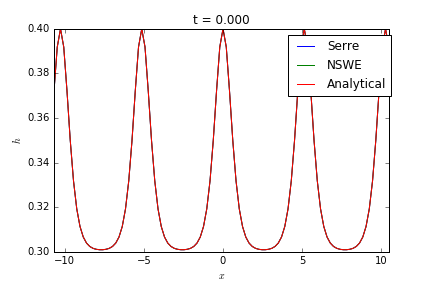
\includegraphics[scale=.3]{figures/Serre/cnoidal1h.png}	
	\end{subfigure}
	\begin{subfigure}{.3\linewidth}
		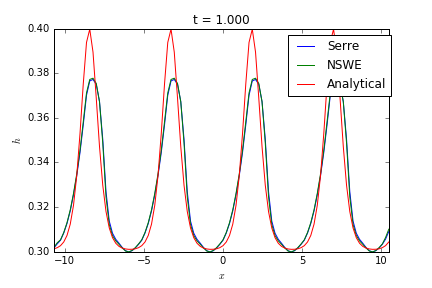
\includegraphics[scale=.3]{figures/Serre/cnoidal2h.png}	
	\end{subfigure}
	\begin{subfigure}{.3\linewidth}
		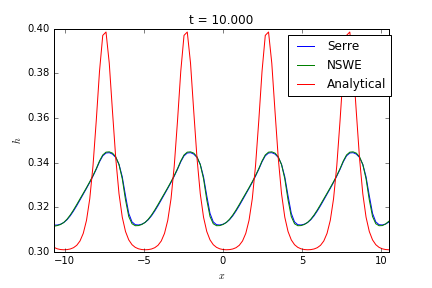
\includegraphics[scale=.3]{figures/Serre/cnoidal3h.png}	
	\end{subfigure}
	\caption{Evolution of $h$ for the cnoidal solution in the Serre equation \label{fig:cnoidalh}}
\end{figure}

\begin{figure}[h!]
	\begin{subfigure}{.3\linewidth}
		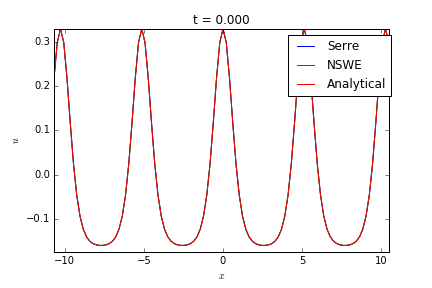
\includegraphics[scale=.3]{figures/Serre/cnoidal1u.png}	
	\end{subfigure}
	\begin{subfigure}{.3\linewidth}
		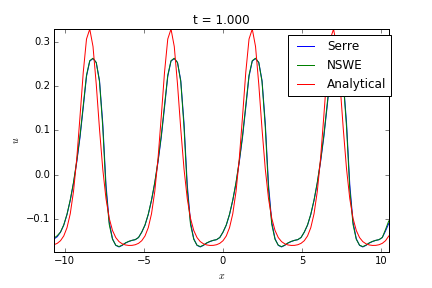
\includegraphics[scale=.3]{figures/Serre/cnoidal2u.png}	
	\end{subfigure}
	\begin{subfigure}{.3\linewidth}
		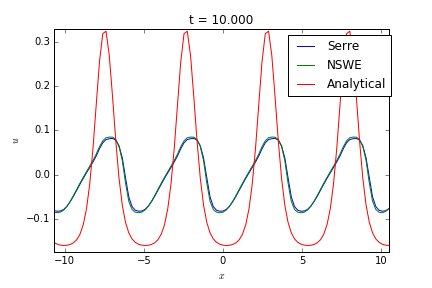
\includegraphics[scale=.3]{figures/Serre/cnoidal3u.png}	
	\end{subfigure}
	\caption{Evolution of $u$ for the cnoidal solution in the Serre equation \label{fig:cnoidalu}}
\end{figure}

\begin{figure}[h!]
	\begin{subfigure}{.3\linewidth}
		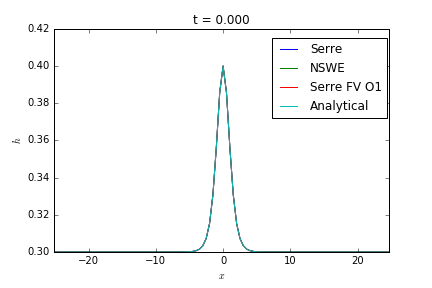
\includegraphics[scale=.3]{figures/Serre/solitary1h.png}	
	\end{subfigure}
	\begin{subfigure}{.3\linewidth}
		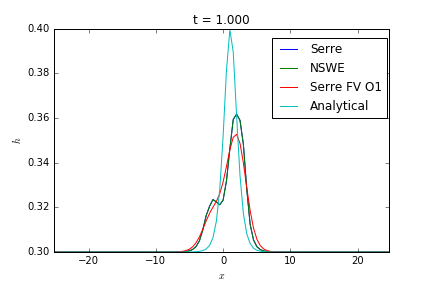
\includegraphics[scale=.3]{figures/Serre/solitary2h.png}	
	\end{subfigure}
	\begin{subfigure}{.3\linewidth}
		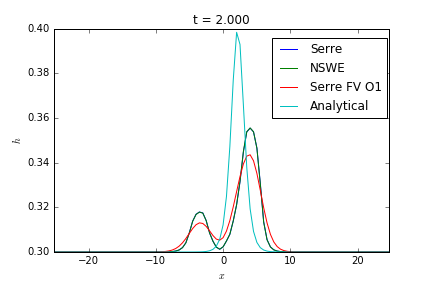
\includegraphics[scale=.3]{figures/Serre/solitary3h.png}	
	\end{subfigure}
	\caption{Evolution of $h$ for the solitary solution in the Serre equation \label{fig:solitaryh}}
\end{figure}

\begin{figure}[h!]
	\begin{subfigure}{.3\linewidth}
		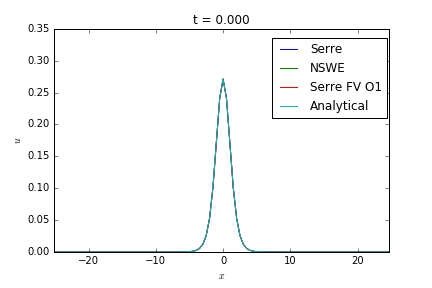
\includegraphics[scale=.3]{figures/Serre/solitary1u.png}	
	\end{subfigure}
	\begin{subfigure}{.3\linewidth}
		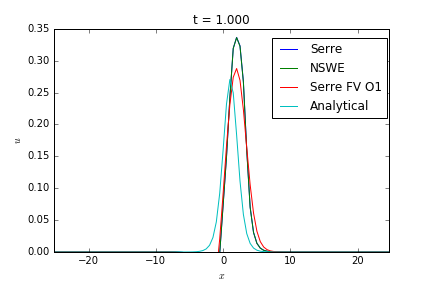
\includegraphics[scale=.3]{figures/Serre/solitary2u.png}	
	\end{subfigure}
	\begin{subfigure}{.3\linewidth}
		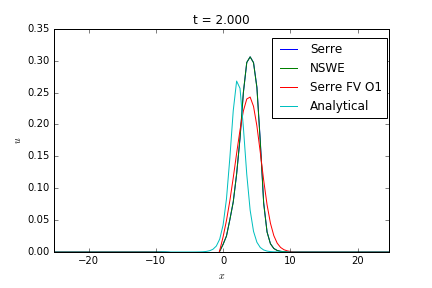
\includegraphics[scale=.3]{figures/Serre/solitary3u.png}	
	\end{subfigure}
	\caption{Evolution of $u$ for the solitary solution in the Serre equation \label{fig:solitaryu}}
\end{figure}

\indent The results show the existence of modeling or programming errors. In both cases tested, the analytical solution is not preserved : we observe a strong dissipation of the solution, and, in the solitary wave case, a inversion of the velocity that causes the formation of secondary waves. The utilization of a higher-order solver for the Finite Volume scheme did not corrected this last problem, but showed a lower dissipation.